\documentclass[../main.tex]{subfiles}


\begin{document}

\section{Introduction}

It is very common that people clone codes in their programs, i.e. reuse some code fragments by copying with or without modification in the coding process. 
Previous research shows a significant fraction of the code being cloned even in some well-known software systems. The fraction of duplicated code in X Windows System is about 19\%\cite{cloneinsys1}, while in some core parts of Linux the number is between 15\% and 25\%\cite{cloneinsys2}. 
Even if code clones can improve the efficiency of a program in some cases, such as remove method calls and reduce execution time, they propose challenges for developers to maintain software: if fixing a bug, adding or removing a feature, it has to be applied to all the similar parts. To solve this problem, clone detection has become an important tool for programmers, since it can help indentify duplicated code when making a change.

There are mainly four types of clones:

\indent \emph{Type 1}: simply includes the variations in whitespace, layout and comments.

\indent \emph{Type 2}: in addition to \emph{Type 1}, it allows more variations in identifiers, literals and types.

\indent \emph{Type 3}: contains \emph{Type 2} and allows further modifications such as changed, added or removed statements. 

An example of \emph{Type 1, 2, 3} clones is shown below:  

\begin{lstlisting}[basicstyle=\footnotesize, language=Java]
public static int Num(int X, int Y){
	int a = 100;
	int b = 200;
	if(X>Y){
		return b + X;
	}
	else{
		a = 80;
		return a + Y;
	}
}

public static int Num(int X, int Y){
	int a=100;
	// no blanks _Type 1
	int c = 120;
	// b to c _Type 2
	if(X>Y){
		X = X - Y;
		// add stmt _Type 3
		return c + X;
	}
	else{
		a = 80;
		return a + Y;
	}
}
\end{lstlisting}

\indent \emph{Type 4}: code fragments perform the same computation or results but are implemented in different ways. 

Few tools have been developed to detect \emph{Type 4} clones so far. 


%\begin{figurehere}
%\centering 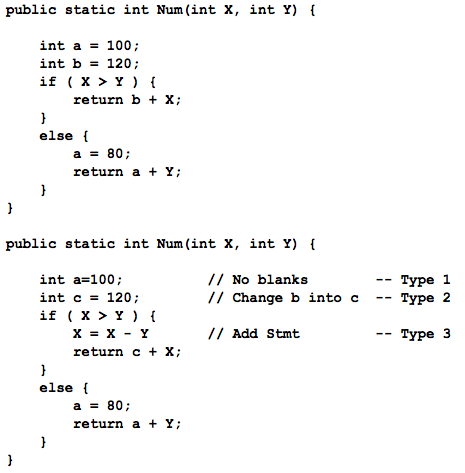
\includegraphics[width = 0.45 \textwidth]{graph2_1} 
%\caption{An example of textual clones} \label{fig:TOC}
%\end{figurehere} 


Based on the clone types, a number of techniques and tools have been implemented. Token-based method shows the best performance among all these techniques. However, each tool has its own limitations, just like the time cost of CCFinder. We propose to develop and implement a scalable clone detection based on tokens to detect code clone in token variation and statement modification.

Our approach is based on the following insight: most developers would not make dramatic changes in code clone process except for some token modifications including keywords, types, variables and operators. 
We try to design and improve a simple statistical method to calculate the similarity between code fragments. 
Specifically, to detect whether fragment A is a clone of fragment B or not, we first tokenize each fragment and design a flexible token filter. Any useful tokens, such as types, variables, identifiers, operators, will be counted, so the information is transformed into a token frequency vector. 
The second step is the pretreatment of variable names, take $v_A$ and $v_B$, compare and find out similar variables with small variations in prefix, suffix and substitution. 
After finding matching variable names, the third step is to use a similarity algorithm to measure the two vectors, by putting different weights on different levels of tokens, and the weights can be set by machine learning, which enhances the accuracy.
Finally, a threshold is introduced and optimized, depending on the precision and recall from actual experiments.

After actual testing, STCD reaches 90\% in both precision and recall rate, which means STCD is very effective. The time cost is quadratic in terms of number of methods in Java file: running a Java file with 100 methods takes only 2 seconds, which is very practical.

The structure of the rest of the paper is as follows: in Section 2, we introduce the mechanism of STCD in detail; in Section 3, we describe the implementation of STCD; in Section 4, we evaluate STCD and get the precision and recall rate, and also the time cost; in Section 5, we analyze the threats to validity; Section 6 is the conclusion; Section 7 lives the related work. 

%Our tool has its own advantages: the first part of this process is just counting, which has very low time cost; the next part is to find out similar variable names, which is the most time-consuming part in our process, but is still not complicated; the last part is to compare token frequency vectors, which is simple math and pretty straightforward. For the whole process, we can expect low time cost.
%
%For a counting based detection tool with low time cost, the accuracy can still be maintained to some extent, in our algorithm, the weighting part does contribute.

Our solution is new and we believe it's aggressive in clone detection field.






\end{document}